%!TEX root = ../../thesis.tex

This introductory chapter provides background reading specific to energy harvesting.
It builds upon the preceding introductory material of double layers and is steered toward energy conversion.
We will discuss how double layers can be used to convert fluid-mechanical power into electrical power.
At this point it is assumed the reader knows what a double layer is and how one is formed.

\section{Streaming Cells}
  \begin{figure}
      \centering
      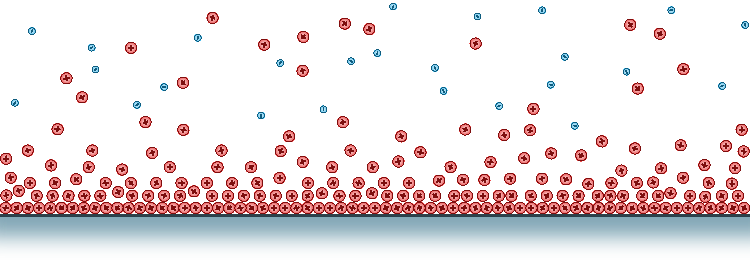
\includegraphics{content/pt1/01-PowerHarvesting/graphics/intro_2_wall}
      \caption{\label{fig:doubleLayerBetweenWalls}Formation of a double layer along a solid wall}
  \end{figure}

  We begin by looking at double layers formed along the walls of a container.
  Such a situation is presented in \ref{fig:doubleLayerBetweenWalls}, where the walls are negatively charged and hence the counter-ions are positive.
  Counter-ions that have been separated from the bulk of the liquid line the exterior of the wall.
  However, charge separation alone is not enough to generate electrical power.

  As energy cannot simply be created or destroyed, it must be converted from one form to another.
  The counter-ions are electrostatically bound to the interface and therefore removing them requires work.
  So although the counter-ion density has been increased at the boundary, the charge is not free.
  Also, the migration of charge to the walls ceases once the surface potential has been neutralised, so it is not a continuous process.

  \begin{figure}
      \centering
      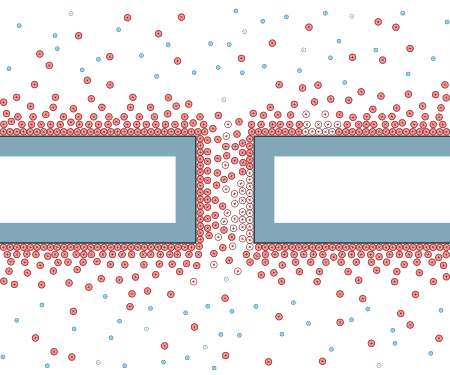
\includegraphics{content/pt1/01-PowerHarvesting/graphics/intro_2_channel_relaxed}
      \caption{\label{fig:doubleLayerInChannel_noPressure}Double layer formation within a streaming cell that is in a state of equilibrium.}
  \end{figure}

  Generating electrical power is going to require using mechanical energy from the fluid.
  This will manifest itself as a drop in pressure across a harvester as liquid is forced through.
  This is similar in nature to the voltage drop observed across an electrical resistor as it passes current.

  The mechanical energy taken from the fluid is used to upset the ionic balance.
  This means separating and isolating negative and positive ions from each other.
  The collection of free (in this case unbound) counter-ions can be achieved by pumping ions from within the double layer out into an isolated region.

  Figure~\ref{fig:doubleLayerInChannel_noPressure} shows another charged wall, but with the addition of a small channel.
  This channel connects two bodies of liquid that have been separated by the wall.
  Notice that the channel contains no co-ions, it is exclusively occupied by counter-ions.
  The ratio of counter-ions to co-ions within the channel is controlled by the width of the channel.
  The narrower the channel, the less likely it is for co-ions to pass.

  Ideally, the width of the channel will be in the order of the double layer thickness.
  The channel depicted in figure~\ref{fig:doubleLayerInChannel_noPressure} is small enough that the double layers will overlap.
  By overlapping the double layers, or bringing their boundaries together, co-ions will be repelled from between the walls.
  This gives rise to highly concentrated counter-ion fluid occupying the channel.

  A channel can be created individually using a range of fabrication methods, such as chemical etching or using narrowly separated parallel plates.
  They can also be formed en-mass by using porous materials such as glass or ceramics, where the pores themselves act as channels.

  The channel and the two separated bodies now form an energy harvester.
  By applying a pressure differential across the channel, counter-ion rich fluid is transported.
  As counter-ions exit the channel on the low-pressure side, new ions move to replenish the double layer on the high-pressure side.
  Once charge has crossed the channel it is difficult for it to return as the constant flow of liquid opposes charge migration back through the wall.
  A diagram showing the channel geometry but with pressure applied and a voltage gradient generated is shown as figure~\ref{fig:doubleLayerInChannel_withPressure}.

  \begin{figure}[ht]
      \centering
      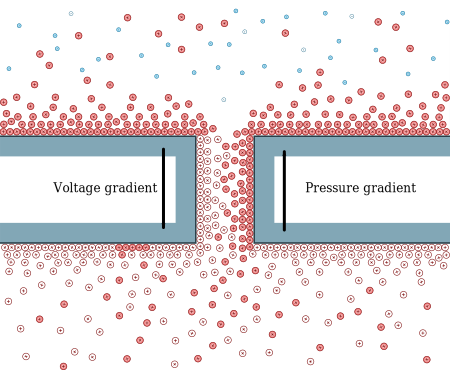
\includegraphics{content/pt1/01-PowerHarvesting/graphics/intro_2_channel}
      \caption{\label{fig:doubleLayerInChannel_withPressure}Double layer formation within a streaming cell that has a pressure differential applied.}
  \end{figure}

  A streaming cell is able to continuously pump ions through its channel.
  Once this process begins, the electrical potential between the two bodies increases.
  Not only is the channel increasing the concentration of free counter ions on the low-pressure side, but it also concentrates co-ions on the high-pressure side.

  Glass has the attractive property that it obtains a negative surface charge when in contact with water.
  This surface charge is caused by the deprotonation of surface silanol groups in glass (SiOH~$\leftrightarrows$~SiO$^{-}+$~H$^{+}$)~\cite{Kirby2004}.
  By immersing a glass channel in an electrolyte solution, double layers of counter-ions (positive ions in this case) occupy the interior walls of the channel.
  This means that the low-pressure side will have a higher potential than that of the high-pressure side, as illustrated throughout the ionic figures.

  The mechanism described here is the streaming potential cell.
  It is a device of interest in both membrane and interface science.
  The concept behind the device is relatively straight-forward, but the physical reality is more complicated.
  The diagrams presented are vastly oversimplified, having perfectly flat walls, single atom ions carrying a single charge, and omitting polar molecules or contaminants.

  This concludes the introduction to Streaming Cells.
  By now you should be comfortable with the concept of using an interfacial double layer to convert mechanical energy through a fluid into electrical energy.
  Next, literature concerning the operation, design and improvements of streaming cell technology is presented.

\section{Literature Review}

  \begin{figure}
    \centering
    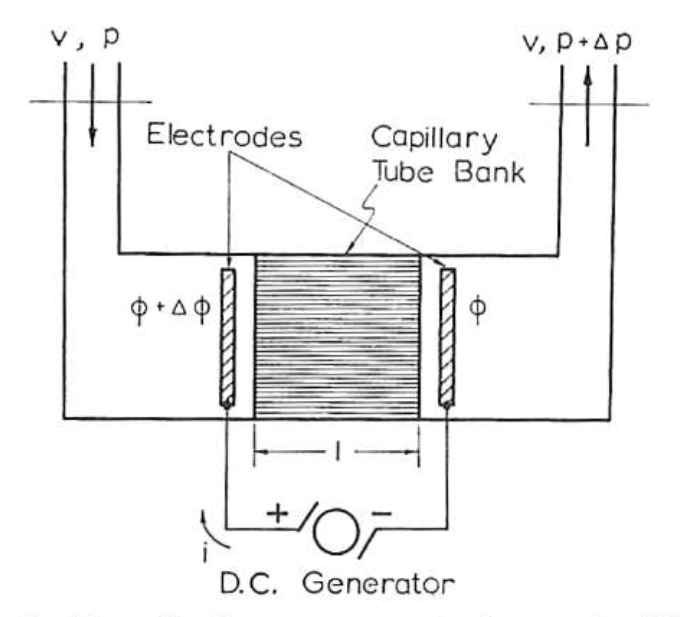
\includegraphics[height=6cm]{content/pt1/Osterle_ElectrokineticCell.png}
    \caption{\label{fig:Osterle_cell}Osterle's electrokinetic pumping cell, reproduced from \cite{Osterle1964}}
  \end{figure}

  In 1964, a paper written by Osterle was published titled ``Electrokinetic Energy Conversion'' \cite{Osterle1964}.
  In that paper Osterle presented an analysis of energy conversion, both for the purpose of pumping or generating electrical power.
  His cell consisted of fine capillary tubes stacked together to form a streaming cell.
  A diagram of that cell, in its pumping configuration, is reproduced from that paper as~\cref{fig:Osterle_cell}.
  Importantly, he shows that a streaming cell has the same conversion efficiency whether it is in a pumping mode, where electrical energy is supplied, or in a generating mode, where electrical energy is produced.

  Based on his analysis, Osterle gives an illustrative example of an streaming cell producing electrical energy.
  He states that tube bank having a volume of \SI{100}{\centi\meter\cubed} with \SI{100}{\kilo\pascal} of hydrostatic pressure applied would be capable of producing \SI{0.49}{\watt} of electrical energy.
  This would require \SI{125}{\watt} of pumping power to achieve, giving an energy conversion efficiency of \SI{0.392}{\percent}.

  In the same year, Burgreen and Nakache publish a paper showing the effect of surface potential on fine capillary tubes, such as those described by Osterle\cite{Burgreen1964}.
  They show that a sufficiently large surface potential will cause flow retardation to approach \SI{100}{\percent}.
  At that point a channel has become impermeable and therefore useless as an energy converter.
  Having a high surface potential is generally desirable as it increases the counter-ion concentration within a channel, however it now seems that such a surface potential would be beyond anything practically obtainable.

  Then, much later, in 2003, Yang et al.\ published in an analysis relating energy conversion efficiency to the length of a streaming cell channel~\cite{Yang2003}.
  The work indicates that short cells are preferable for efficient electrical generation.

  In 2004, Daiguji et al.\ report on the relationship between the Debye length of the double layer and a streaming cells conversion efficiency~\cite{Daiguji2004}.
  They find that a channel is most efficient when its height is twice that of the Debye length.
  This corresponds to the point at which formed double layers within a channel begin to overlap.

  In 2005, van der Heyden et al.\ reports on streaming cell measurements made in a single microchannel \SI{70}{\micro\meter} in height~\cite{VanderHeyden2005}.
  Many valuable contributions were detailed in this paper, namely:
  \begin{enumerate}
    \item Confirmed that reversing the polarity of surface potential reverses the direction of the streaming current.
    \item Found that the maximum conversion efficiency corresponded to channels where double layers begin to overlap. This confirms the relationship put forward the previous year by Daiguji et al.\
    \item Show that boundary conditions involving constant surface potentials, used up to this point to model streaming, are inaccurate.
    \item Predict a maximum energy conversion efficiency of $\sim$\SI{6}{\percent} for potassium chloride solutions of \SI{1e-5}{\mole} in silica channels of height \SI{145}{\nano\meter}.
  \end{enumerate}

  In 2006, van der Heyden et al.\ publishes a follow-up to their previous work~\cite{VanderHeyden2006}.
  They calculate that energy conversion efficiency is maximised at low salt concentrations.
  And, they make a prediction of \SI{12}{\percent} efficiency for streaming cells utilising a lithium based ions in solutions.

  Also in 2006, Daiguji et al.\ publish work suggesting that in order to increase cell efficiency one may either reduce the channel height or decrease the ionic concentration of the working fluid~\cite{Daiguji2006}.
  This supports the work of van der Heyden et al.\ with respect to efficiency gains with the working fluids having low ionic concentrations.

  In 2007, van der Heyden et al.\ publish a measured energy conversion of \SI{3.2}{\percent}~\cite{Heyden2007}.
  They suggest that the conversion efficiency of a channel is limited by a property termed `Stern conductance'.
  The concept of stern conductance is that the stern layer (see \cref{fig:doubleLayer_anatomy}) itself provides a pathway for electrical conduction.
  Stern conductance is often referred simply as `surface conductance', and is a property that will be estimated based on measurements of fabricated cells in proceeding chapters.

  That same year an article written by Pennathur, Eijkel, and Berg reported results from a mathematical model predicting the effects of hydrodynamic slip~\cite{Pennathur2007}.
  It proposed efficiency figures as high as \SI{30}{\percent} for a slip length of \SI{6.5}{\nano\meter} in cylindrical tubes \SI{100}{\nano\meter} in diameter.

  \begin{figure}
    \centering
    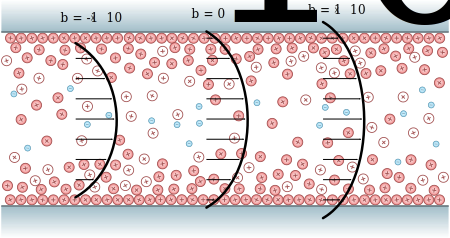
\includegraphics[height=6cm]{content/pt1/graphics/HydrodynamicSlip}
    \caption{\label{fig:HydrodynamicSlip}Illustration of hydrodynamic slip inside a channel cavity, where $b$ is the slip length. Arrows indicate flow velocity in each of the three situations.}
  \end{figure}

  Hydrodynamic slip refers to the ability of a fluid to `slip' relative to a boundary/interface.
  Slip is advantageous as it allows the transport of ions in the Stern layer (where the counter-ion concentration is highest).
  The length refers to an imaginary distance into the solid wall where the traditional `no-slip' boundary condition would occur (refer to~\cref{fig:HydrodynamicSlip}).
  The `no-slip' boundary condition states that at the boundary between solid and fluid, a fluid has no velocity.
  This condition, along with viscosity, produces the parabolic flow profile as fluid moves through pipes.

  In a separate article, but in the same journal, Eijkel discusses the relationship between zeta potential and slip length~\cite{Eijkel2007}.
  The general problem with slip based mechanisms is that a high zeta potential is optimal for double layer formation, however it also promotes wetting.
  This surface wetting is what causes the no-slip boundary condition in the first place.
  In order to improve the situation in steaming cells a surface should be both non-wetting and hold a high surface charge.

  The following year (2008), Davidson and Xuan publish a mathematical model confirming the role of Stern conductance on streaming cells, in particular those with low ionic strength~\cite{Davidson2008}.
  They suggest that this is the reason for poor measured efficiencies in light of the much higher predicted values.

  \begin{figure}
    \centering
    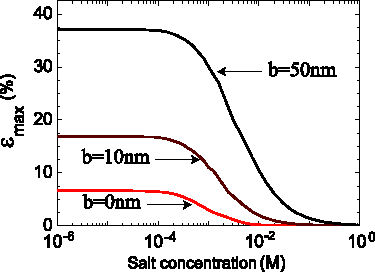
\includegraphics[height=6cm]{content/pt1/graphics/SteinSlipEnchancedChannelEfficiency}
    \caption{\label{fig:Stein_Slip_Prediction}Plot of predicted efficiency versus salt concentration for various for slip lengths of 0, 10 and \SI{50}{\nano\meter}, taken from~\cite{Ren2008}.}
  \end{figure}

  That same year, two papers modelling the effects of hydrodynamic slippage were published.
  The first, by Davidson and Xuan, gives a mathematical prediction of the effects of hydrodynamic slippage at the interface surface~\cite{Davidson2008a}.
  They predict that when taking slip at the solid-fluid boundary into consideration that conversion efficiencies as high as \SI{30}{\percent} should be obtainable.

  The second, by Ren and Stein, predict conversion efficiencies as high as \SI{70}{\percent} based on the slip lengths recently observed with carbon nanotubes~\cite{Ren2008}.
  They provide a more conservative prediction of \SI{40}{\percent} for slip lengths in the tens of nanometers region and low salt concentration.

  In 2009, Chang and Yang, publish a Poisson-Boltzmann based model of streaming cells showing a decrease in conversion efficiency at maximum power when the channel length is low~\cite{Chang2009}.
  This work suggests there is an optimum channel length, which is also dependant on the fluid conductivity.

  By this time there have been numerous conversion efficiencies reported in the literature.
  These are summarised as follows:
  \begin{itemize}
    \item ``far less than \SI{1}{\percent}'' forcing potassium chloride through a porous glass plug having pores in the range \SI{1}--\SI{1.6}{\micro\meter}~\cite{Olthuis2005}.
    \item 0.01\% by forcing water through porous glass with pore sizes from 10\thinspace--\SI{16}{\micro\metre}.~\cite{Yang2003}
    \item 0.8\% by forcing pure water through a ceramic rod populated with \SI{6}{\micro\metre} pores.~\cite{Yang2004}
    \item 3\% by forcing a sodium chloride solution through a \SI{75}{\nano\metre} by \SI{50}{\micro\metre} silica channel.~\cite{Heyden2007}
    \item 0.77\% by forcing a sodium chloride solution through a \SI{200}{\nano\metre} pore in an alumina membrane.~\cite{Lu2006}
    \item 5\% by forcing a sodium chloride solution through a \SI{0.5}{\nano\metre} cylindrical pore in polyethylene terephalate foil.~\cite{Xie2008}
  \end{itemize}

  In 2012, Cherng Hon et al.\ presented a novel method of producing electrokinetic power from steaming cells using salinity gradients~\cite{CherngHon2012}.
  In this work the authors describe a system where flow through a conventional streaming cell is brought about by forward osmosis.
  This allows the authors to generate electrical energy from streaming cells without mechanical pumping.
  The application has limited use, but it highlights novel uses for streaming cells as a means of electrical generation.

  Recently, in 2014, Jiao et al.\ presented results showing that surface treatment of porous glass can increase conversion efficiency~\cite{Jiao2014}.
  They show that ultrasonically pre-treating glass and subsequently applying Sodium Dodecyl Sulphate to the surface gave a relative increase of \SI{27.3}{\percent} in power density.
  Unfortunately, they do not state the absolute efficiency of their channels in either case.


  Theoretical predictions of the efficiency of standard micro/nano-fluidic channels are 2\% for pure water and 7\% for sodium chloride.~\cite{VanderHeyden2006}
  Experimental results show conversion efficiencies in the range of:
  These results indicate that small channels using solutions containing salt are more efficient.
  According to \cite{Daiguji2004}, the efficiency is maximised when the channel height twice that of the Debye length.
  Additionally, ~\cite{VanderHeyden2006} states that the maximum efficiency is found when the salt concentration is low.

  It is clear from the literature that there is significant progress to be made with respect to increasing the conversion efficiency of streaming cells.
  Techniques to induce hydrodynamic slip at the fluid-solid interface are predicted to increase this efficiency to 30-40\%~\cite{Davidson2008a, Ren2008}, but progress in this area is dictated by advancements in materials science.
  Experimental results utilising slip enhanced channels have not yet been reported in the literature.
  Surface enhanced channels will not be investigated due to manufacturing difficulty, cost, and the level of scientific development required to make progress.

  The finding that maximum conversion efficiency occurs when ionic concentration is low supports the use of tap-water as a working fluid.
  The use of glass as a substrate appears to be a suitable choice, which is both cost effective and a convenient material.
  The dimensions of cells found in the literature suggest that we could fabricate trial cells.
